% interpolacion_bicuadrada_R_completo_tikz.tex
% Figura completa de interpolación bicuadrada para canal R (fórmulas con espaciado uniforme)

\begin{figure}[H]
\centering
\begin{tikzpicture}[
    font=\normalsize,
    cell/.style={rectangle, draw=black, minimum size=1.2cm, inner sep=0},
    legendcell/.style={rectangle, draw=black, minimum size=0.8cm, inner sep=0},
    formula/.style={font=\footnotesize, align=left}
]

% ============================================
% PARÁMETROS DE LA CUADRÍCULA
% ============================================
\def\gridWidth{14}   % Ancho total aumentado (en cm)
\def\rowOneHeight{3.5}  % Alto de la fila 1 (en cm)
\def\rowTwoHeight{3}    % Alto de la fila 2 (en cm)
\def\colWidth{2.8}    % Ancho de cada columna (en cm)

% ============================================
% DEFINICIÓN DE COORDENADAS DE CENTRO
% ============================================
% Fila 1 (ahora con 5 columnas para más espacio)
\coordinate (F1C1) at (0.5*\colWidth, 0);
\coordinate (F1C2) at (1.5*\colWidth, 0);
\coordinate (F1C3) at (2.5*\colWidth, 0);
\coordinate (F1C4) at (3.5*\colWidth, 0); % Espacio extra
\coordinate (F1C5) at (4.5*\colWidth, 0); % Leyenda más a la derecha

% Fila 2 (ocupa ancho completo de 5 columnas)
\coordinate (F2) at (2.5*\colWidth, -\rowOneHeight-0.5*\rowTwoHeight);

% ============================================
% F1C1: MATRIZ ORIGINAL - CANAL R
% ============================================
\begin{scope}[shift={(F1C1)}]
    % Título
    \node[above, font=\bfseries, red!80!black] at (0, 1.8) {Canal R Original};
    
    % Matriz 3x3
    % Fila 1
    \node[cell, fill=red!80!black] at (-1.2, 1.2) {\textcolor{white}{$r_{11}$}};
    \node[cell, fill=gray!20] at (0, 1.2) {$0$};
    \node[cell, fill=red!80!black] at (1.2, 1.2) {\textcolor{white}{$r_{13}$}};
    
    % Fila 2
    \node[cell, fill=gray!20] at (-1.2, 0) {$0$};
    \node[cell, fill=gray!20] at (0, 0) {$0$};
    \node[cell, fill=gray!20] at (1.2, 0) {$0$};
    
    % Fila 3
    \node[cell, fill=red!80!black] at (-1.2, -1.2) {\textcolor{white}{$r_{31}$}};
    \node[cell, fill=gray!20] at (0, -1.2) {$0$};
    \node[cell, fill=red!80!black] at (1.2, -1.2) {\textcolor{white}{$r_{33}$}};
\end{scope}

% ============================================
% F1C2: FLECHA DE PROCESO
% ============================================
\begin{scope}[shift={(F1C2)}]
    \node[font=\Huge] at (0, 0) {$\Rightarrow$};
    \node[above, font=\scriptsize] at (0, 1) {Interpolación};
    \node[below, font=\scriptsize] at (0, -1) {Bicuadrada};
\end{scope}

% ============================================
% F1C3: MATRIZ INTERPOLADA - CANAL R
% ============================================
\begin{scope}[shift={(F1C3)}]
    % Título
    \node[above, font=\bfseries, red!80!black] at (0, 1.8) {Canal R Interpolado};
    
    % Matriz 3x3 completa
    % Fila 1
    \node[cell, fill=red!80!black] at (-1.2, 1.2) {\textcolor{white}{$r_{11}$}};
    \node[cell, fill=red!60!black] at (0, 1.2) {\textcolor{white}{$r_{12}$}};
    \node[cell, fill=red!80!black] at (1.2, 1.2) {\textcolor{white}{$r_{13}$}};
    
    % Fila 2
    \node[cell, fill=red!60!black] at (-1.2, 0) {\textcolor{white}{$r_{21}$}};
    \node[cell, fill=red!40!black] at (0, 0) {\textcolor{white}{$r_{22}$}};
    \node[cell, fill=red!60!black] at (1.2, 0) {\textcolor{white}{$r_{23}$}};
    
    % Fila 3
    \node[cell, fill=red!80!black] at (-1.2, -1.2) {\textcolor{white}{$r_{31}$}};
    \node[cell, fill=red!60!black] at (0, -1.2) {\textcolor{white}{$r_{32}$}};
    \node[cell, fill=red!80!black] at (1.2, -1.2) {\textcolor{white}{$r_{33}$}};
\end{scope}

% ============================================
% F1C5: LEYENDA DE COLORES (AJUSTADA VERTICALMENTE)
% ============================================
\begin{scope}[shift={(F1C5)}]
    % Título
    \node[above, font=\bfseries] at (0, 1.8) {Leyenda de Colores};
    
    % Ajuste: movemos toda la leyenda 0.8cm hacia arriba
    \def\verticalShift{0.8}
    
    % Original (rojo oscuro)
    \node[legendcell, fill=red!80!black] at (-1, 0.5+\verticalShift) {};
    \node[anchor=west, font=\small] at (-0.7, 0.5+\verticalShift) {Original};
    \node[anchor=west, font=\tiny] at (-0.7, 0.2+\verticalShift) {($r_{11}$, $r_{13}$, $r_{31}$, $r_{33}$)};
    
    % Interpolado 1D (rojo medio)
    \node[legendcell, fill=red!60!black] at (-1, -0.3+\verticalShift) {};
    \node[anchor=west, font=\small] at (-0.7, -0.3+\verticalShift) {Interpolado 1D};
    \node[anchor=west, font=\tiny] at (-0.7, -0.6+\verticalShift) {($r_{12}$, $r_{21}$, $r_{23}$, $r_{32}$)};
    
    % Interpolado 2D (rojo claro)
    \node[legendcell, fill=red!40!black] at (-1, -1.1+\verticalShift) {};
    \node[anchor=west, font=\small] at (-0.7, -1.1+\verticalShift) {Interpolado 2D};
    \node[anchor=west, font=\tiny] at (-0.7, -1.4+\verticalShift) {($r_{22}$)};
    
    % Por interpolar (gris)
    \node[legendcell, fill=gray!20] at (-1, -1.9+\verticalShift) {};
    \node[anchor=west, font=\small] at (-0.7, -1.9+\verticalShift) {Por interpolar};
    \node[anchor=west, font=\tiny] at (-0.7, -2.2+\verticalShift) {(valor 0)};
\end{scope}

% ============================================
% F2: FÓRMULAS DE INTERPOLACIÓN CON ESPACIADO UNIFORME
% ============================================
\begin{scope}[shift={(F2)}]
    % Título
    \node[above, font=\bfseries] at (0, 1.5) {Fórmulas de Interpolación Bicuadrada};
    
    % Parámetros para el espaciado uniforme
    \def\formulaStartY{0.8}      % Coordenada Y inicial
    \def\formulaSpacing{0.7}     % Espaciado uniforme entre fórmulas
    \def\leftColumnX{-4}         % Columna izquierda
    \def\rightColumnX{2}         % Columna derecha (separada 6cm de la izquierda)
    
    % Columna izquierda: 3 fórmulas
    \node[anchor=north west, formula] at (\leftColumnX, \formulaStartY) 
        {$r_{12} = \tfrac{3}{8}r_{11} + \tfrac{3}{4}r_{13} - \tfrac{1}{8}r_{15}$};
    
    \node[anchor=north west, formula] at (\leftColumnX, \formulaStartY - \formulaSpacing) 
        {$r_{21} = \tfrac{3}{8}r_{11} + \tfrac{3}{4}r_{31} - \tfrac{1}{8}r_{51}$};
    
    \node[anchor=north west, formula] at (\leftColumnX, \formulaStartY - 2*\formulaSpacing) 
        {$r_{22} = \tfrac{9}{64}r_{11} + \tfrac{9}{32}r_{13} + \tfrac{9}{32}r_{31} + \tfrac{9}{16}r_{33} - \tfrac{3}{64}r_{15} - \tfrac{3}{64}r_{51}$};
    
    % Columna derecha: 2 fórmulas (alineadas con las dos primeras de la izquierda)
    \node[anchor=north west, formula] at (\rightColumnX, \formulaStartY) 
        {$r_{23} = \tfrac{3}{8}r_{13} + \tfrac{3}{4}r_{33} - \tfrac{1}{8}r_{53}$};
    
    \node[anchor=north west, formula] at (\rightColumnX, \formulaStartY - \formulaSpacing) 
        {$r_{32} = \tfrac{3}{8}r_{31} + \tfrac{3}{4}r_{33} - \tfrac{1}{8}r_{35}$};
    
    % Línea vertical divisoria (opcional, para referencia)
    \draw[gray!30, dashed] (\leftColumnX + 3, \formulaStartY + 0.2) -- (\leftColumnX + 3, \formulaStartY - 2*\formulaSpacing - 0.2);
\end{scope}

% ============================================
% LÍNEA DIVISORIA HORIZONTAL
% ============================================
\draw[gray!40, thick] (0.2, -\rowOneHeight+0.2) -- (\gridWidth-0.2, -\rowOneHeight+0.2);

\end{tikzpicture}
\caption{Interpolación bicuadrada para el canal rojo (R) en patrón Bayer. Arriba se muestra la transformación de la matriz original (con valores conocidos en rojo oscuro y ceros en gris) a la matriz interpolada (todos los valores completos, diferenciando entre originales, interpolados 1D e interpolados 2D). La leyenda, alineada verticalmente con las matrices, explica los colores utilizados. Debajo se presentan las fórmulas de interpolación bicuadrada con espaciado uniforme, distribuidas en dos columnas para una presentación clara y ordenada.}
\label{fig:interpolacion_bicuadrada_R_completa}
\end{figure}
